\chapter{HPV in Spain}\label{HPVSpain}
In this Chapter, we are going to apply the model to the Spanish scenario. First, we will study the decline of HPV LR infections and, as a consequence, the decline of genital warts. Furthermore, we will study the decline of HPV HR.

Also, we will simulate the hypothetic case when the effect of the vaccine disappears suddenly after 20 years of the vaccination and we will study if the herd immunity remains or changes. 

Moreover, we will assume an infection increases due to the tourism and we will study in which way it affects the infection in the Spanish people and the herd immunity. 

\section{Decline of HPV LR infections and cases of genital warts in the long-term in Spain}
Let us study the decline of HPV LR infections and, consequently, of cases of genital warts in the long-term in Spain. We are going to use the procedure explained in Section \ref{sec:decline}. The vaccination program started in Oct 2007.

The results can be seen in Figure \ref{fig:verrESP}. For women, we also include the percentage of vaccinated women that will help us to visualize the herd immunity effect, because this effect arises when the decline line is over the vaccination line. To be precise, the herd immunity is present, in average, from $2008.3$ ($0.6$ years after the starting of the vaccination program) with CI$95\%$ $[2007.75, 2037.83]$, that is, in the worst case, the herd immunity effect in women will start in $2037.83$, $30$ years after the starting of the vaccination program. 

In case of men, the herd immunity appears from the very beginning $0.58$ year with CI$95\%$ $[0.0, 2.17]$. As men are not vaccinated, the herd immunity can be visualized if the line is over the blue horizontal line. 

The herd immunity in MSM does not exist. There is an almost constant band between $-25\%$ and $20\%$ gathering the best and worst decline percentages with non appreciable changes.

\begin{figure}[!]
	\centering
	\begin{tabular}{cc}
		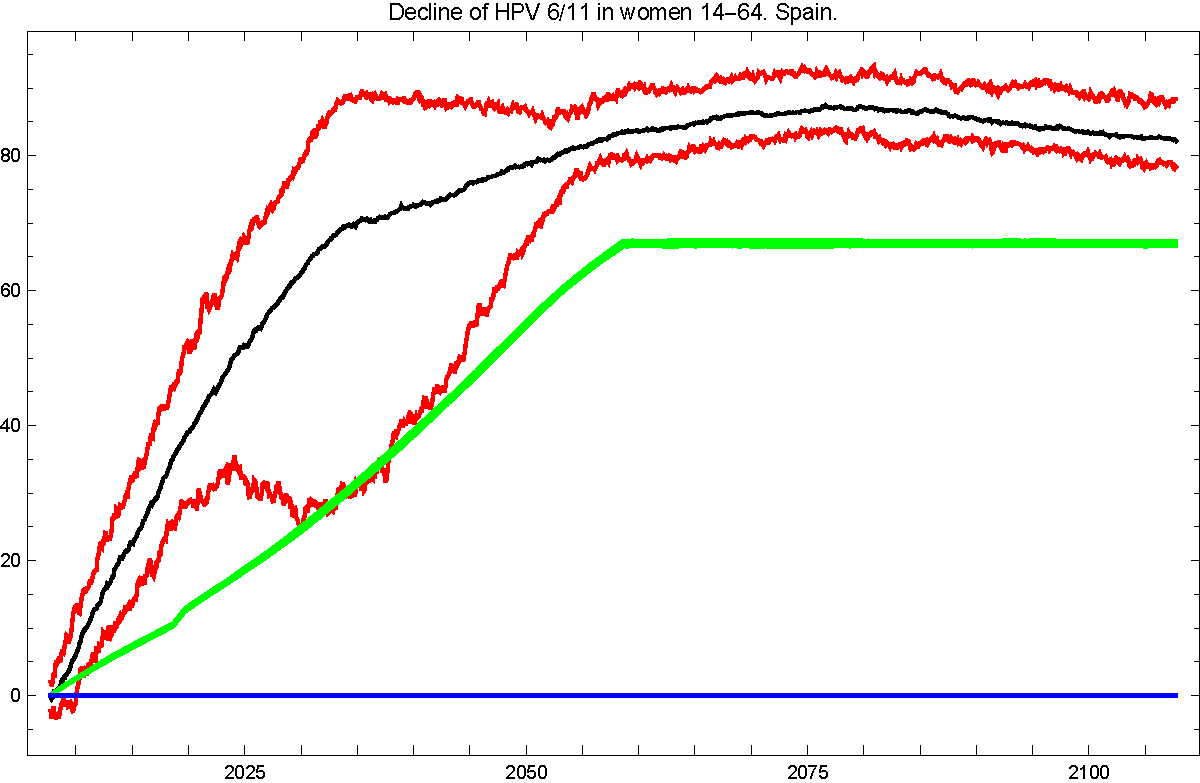
\includegraphics[width=0.5\linewidth]{IMGs/4.-Spain/Decl_muj_14_64_verr_ESP.pdf}	& 
		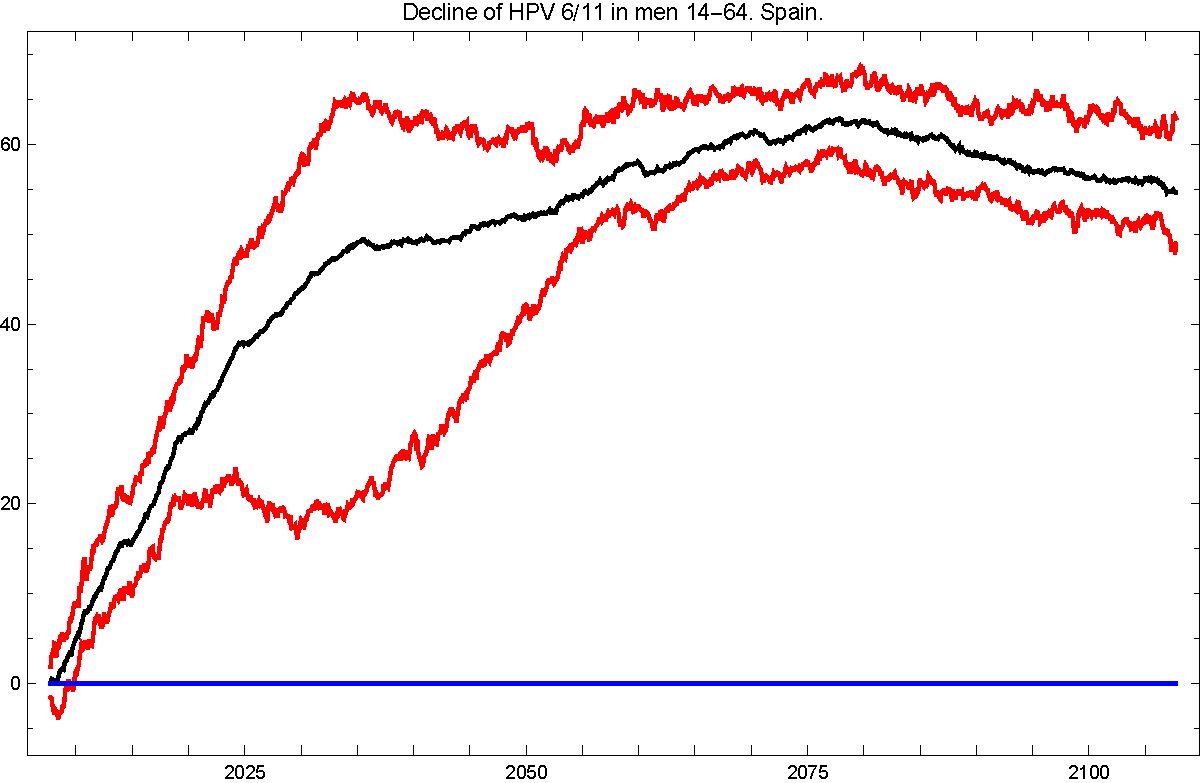
\includegraphics[width=0.5\linewidth]{IMGs/4.-Spain/Decl_hom_14_64_verr_ESP.pdf}  \\ 
		(a)	& (b) \\ 
		\multicolumn{2}{c}{ 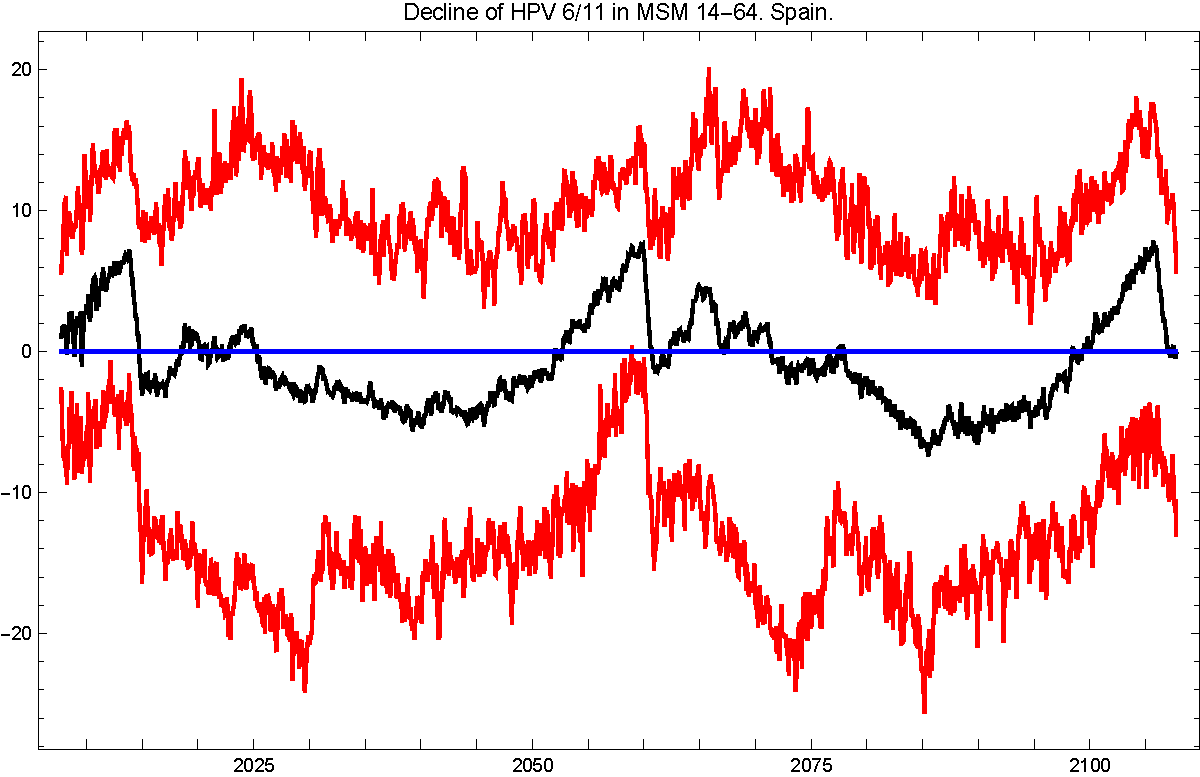
\includegraphics[width=0.5\linewidth]{IMGs/4.-Spain/Decl_MSM_14_64_verr_ESP.pdf} } \\ 
		\multicolumn{2}{c}{(c)} \\ 
	\end{tabular} 
	\caption{Decline of HPV LR 6/11 infections, and consequently, of genital warts (GW) in 14-64 years old women (a), men (b) and MSM (c) over the time, from Oct 2007 when the vaccination campaign started in Spain. In the women decline, we include the percentage of vaccinated women. It helps to visualize the herd immunity effect when the decline line is over the vaccination line. In case of men, the lines over the blue abscissa line means effect of the herd immunity. However, for the MSM, as in the Australian case, there is not herd immunity effect.}
	\label{fig:verrESP}
\end{figure}

The differences between the best and the worst cases is due to the LSP network structure. We do not know exactly how these networks are and the uncertainty that involves the building of these networks may lead to extreme scenarios. This happens in general and in MSM in particular. Thus, we should say that, in our built networks of $100,000$ nodes, less than $2,000$ are labeled MSM. This figure is very low to state predictions for MSM population with a reliable uncertainty and it may explain why the Figure \ref{fig:verrESP} for MSM has so extreme $95\%$ confidence interval.

In the Table \ref{tabla:verrESP}, we can see when given percentages of decline will be reached for women and men. Note that it is not necessary a long time to achieve high percentages of decline for women and men.

\begin{table}[!h]
\centering
\begin{tabular}{c|ll}
	Decline & Women & Men  \\ 
	\hline 
$ 30 \%$ & year  2017 , CI95\% $[ 2015 , 2035 ]$ & year  2021 , CI95\% $[ 2018 , 2044 ]$  \\
$ 40 \%$ & year  2021 , CI95\% $[ 2017 , 2039 ]$ & year  2027 , CI95\% $[ 2023 , 2049 ]$  \\	
$ 50 \%$ & year  2024 , CI95\% $[ 2020 , 2045 ]$ & year  2044 , CI95\% $[ 2027 , 2103 ]$  \\
$ 60 \%$ & year  2029 , CI95\% $[ 2023 , 2047 ]$ & year  2068 , CI95\% $[ 2055 , - ]$  \\
$ 70 \%$ & year  2035 , CI95\% $[ 2027 , 2052 ]$ & year  $-$ , CI95\% $[ - , - ]$  \\
$ 80 \%$ & year  2053 , CI95\% $[ 2030 , 2101 ]$ & year  $-$ , CI95\% $[ - , - ]$  \\
\end{tabular} 
\caption{In this table we show when given percentages of decline of HPV LR 6/11 will be reached over the time with a $95\%$ confidence interval. The symbol "$-$" means that this percentage is not reached in the simulation period. Note that, in average, high percentages of decline for women and men are achieved very soon.}
\label{tabla:verrESP}
\end{table}

\section{Decline of HPV oncogenic HR infections in the long-term in Spain}
Here, we are going to repeat the study done in the previous section corresponding to HPV oncogenic HR 16/18/31/33/45/52/58, those GARDASIL9 protects. In this case, the study may give an idea about the future decline of the cases of HPV-related cancer, but taking into account that cancer use to appear after around $20$ years of persistent infection. 

As in the previous section, we are going to use the procedure explained in Section \ref{sec:decline}. The vaccination program started in Oct 2007.

The results can be seen in Figure \ref{fig:oncoESP}. For women, the herd immunity is present, in average, from $2010$ ($2$ years after the starting of the vaccination program). In the worst case, the herd immunity effect in women appears clearly after $39$ years, around $2047$.

In case of men, in average, the herd immunity appears from the very beginning ($0$ years, $2007.75$). As men are not vaccinated, the herd immunity can be visualized if the line is over the blue horizontal line. In the worst case, $2.5$ years ($2010.25$) are necessary to arise the threshold of the herd immunity.  

As in the previous cases, herd immunity effect does not appear for MSM.

\begin{figure}[!]
	\centering
	\begin{tabular}{cc}
		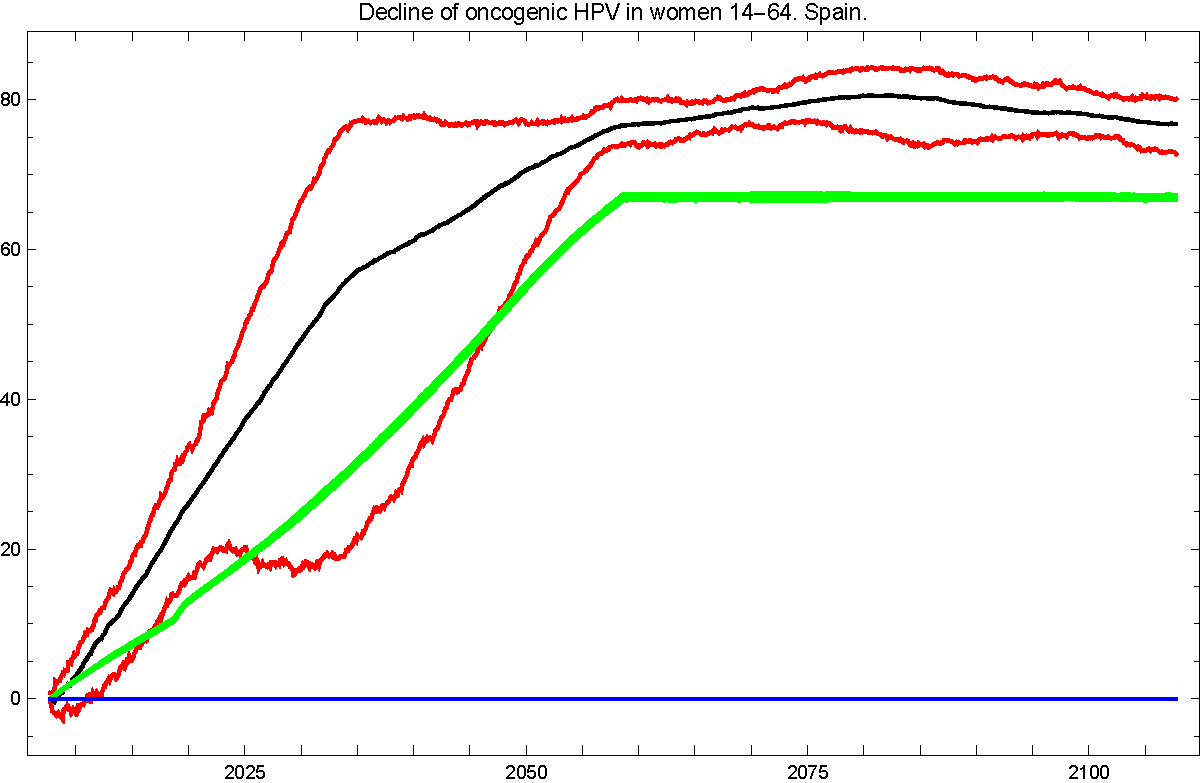
\includegraphics[width=0.5\linewidth]{IMGs/4.-Spain/Decl_muj_14_64_onco_ESP.pdf}	& 
		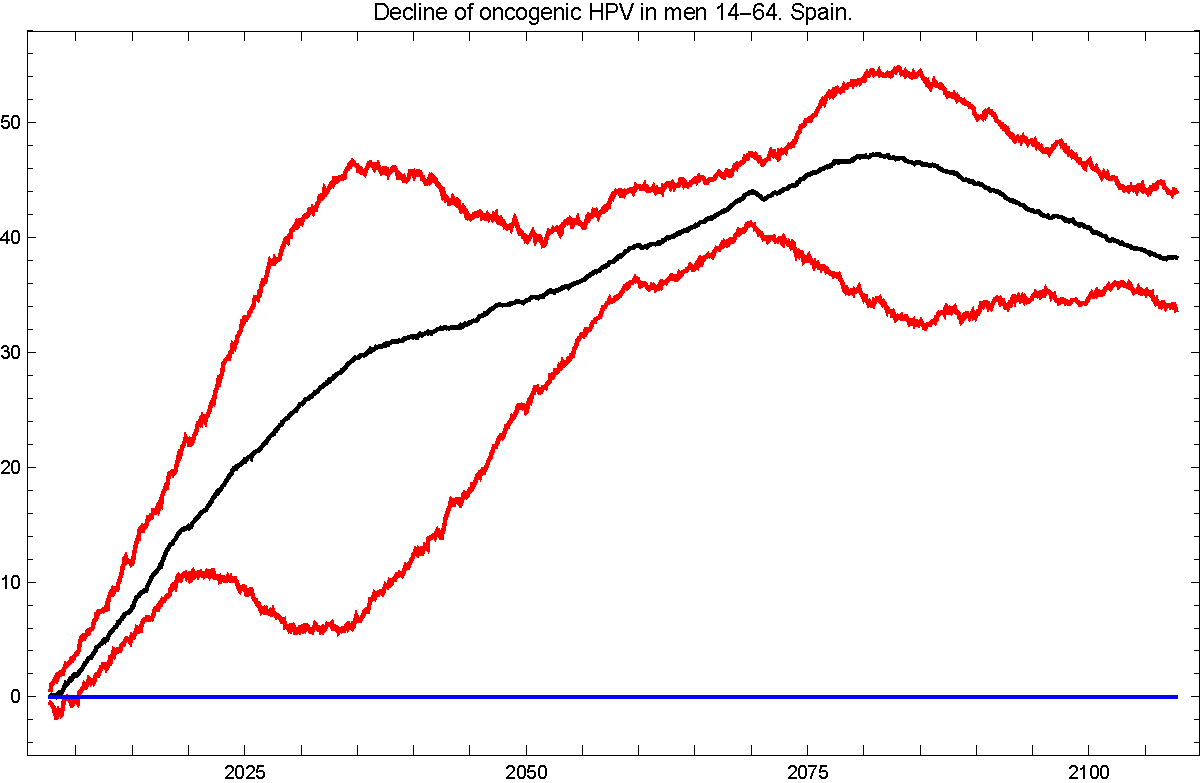
\includegraphics[width=0.5\linewidth]{IMGs/4.-Spain/Decl_hom_14_64_onco_ESP.pdf}  \\ 
		(a)	& (b) \\ 
		\multicolumn{2}{c}{ 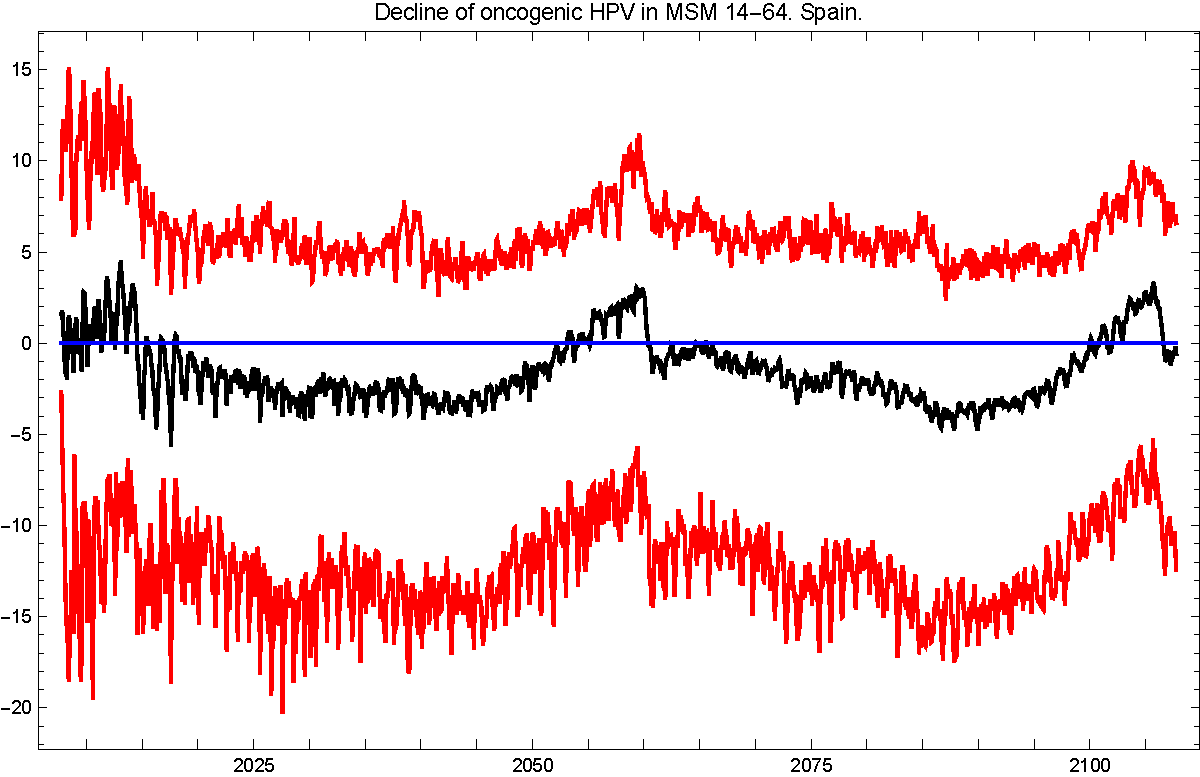
\includegraphics[width=0.5\linewidth]{IMGs/4.-Spain/Decl_MSM_14_64_onco_ESP.pdf} } \\ 
		\multicolumn{2}{c}{(c)} \\ 
	\end{tabular} 
	\caption{Decline of HPV oncogenic HR infections in 14-64 years old women, men and MSM over the time, from Oct 2007, when the vaccination campaign started in Spain. In the women decline, we include the percentage of vaccinated women. It helps to visualize the herd immunity effect when the decline line is over the vaccination line. In case of men, the lines over the blue abscissa line means effect of the herd immunity. For the MSM, there is not herd immunity effect.}
	\label{fig:oncoESP}
\end{figure}

In the Table \ref{tabla:oncoESP}, we can see when given percentages of decline of HPV oncogenic HR will be reached for women and men. As in the HPV LR case, it is not necessary a long time to achieve high percentages of decline for women and men. In fact, the decline percentages for HR oncogenic HR types are better than HPV LR 6/11.

\begin{table}[!h]
	\centering
	\begin{tabular}{c|ll}
		Decline & Women & Men \\ 
		\hline 
$ 30 \%$ & year  2022 , CI95\% $[ 2019 , 2040 ]$ & year  2036 , CI95\% $[ 2024 , 2054 ]$  \\
$ 40 \%$ & year  2027 , CI95\% $[ 2023 , 2044 ]$ & year  2063 , CI95\% $[ 2052 , 2072 ]$  \\
$ 50 \%$ & year  2031 , CI95\% $[ 2025 , 2047 ]$ & year  $-$ , CI95\% $[ 2075 , - ]$  \\
$ 60 \%$ & year  2039 , CI95\% $[ 2028 , 2051 ]$ & year  $-$ , CI95\% $[ - , - ]$  \\
$ 70 \%$ & year  2050 , CI95\% $[ 2032 , 2055 ]$ & year  $-$ , CI95\% $[ - , - ]$  \\
$ 80 \%$ & year  2076 , CI95\% $[ 2108 , - ]$ & year  $-$ , CI95\% $[ - , - ]$  \\
    \end{tabular} 
	\caption{In this table we show when given percentages of decline of HPV oncogenic HR in Spain with the current vaccination program will be reached over the time with a $95\%$ confidence interval. The symbol "$-$" means that this percentage is not reached in the simulation period. }
	\label{tabla:oncoESP}
\end{table}

\section{What would happen in Spain if, after 20 years of the vaccination, the effect of the vaccine disappear completely?}
In this section, we are going to simulate what would happen if the vaccine is protecting completely the vaccinated woman during $20$ years and suddenly, in the month after these $20$ year, she losses completely the protection and she becomes vulnerable to the HPV LR 6/11 and HPV oncogenic HR. In Figure \ref{fig:perdida_proteccion} we can see the evolution of the protection simulated for every vaccinated woman.

\begin{figure}[h!]
	\centering
	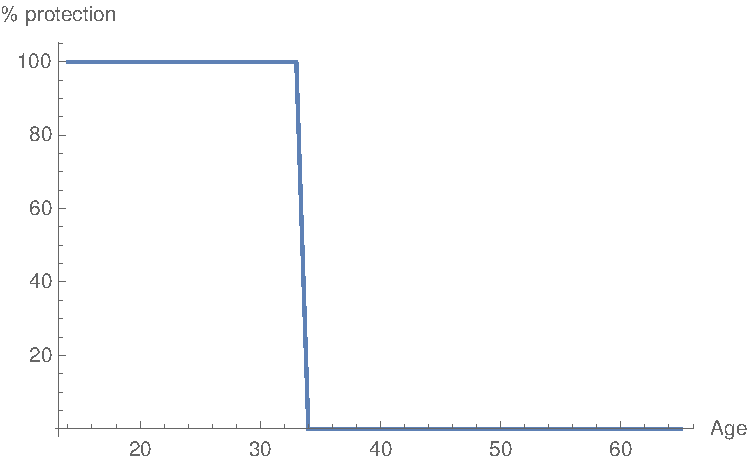
\includegraphics[width=0.5\linewidth]{IMGs/5.-Caida_brusca/grafica_perdida_proteccion.pdf}
	\caption{Evolution of the vaccine protection for every vaccinated woman. After vaccination until $20$ years, the vaccine protects completely ($100\%$) but the month after, the protection drops to $0\%$, the vaccine does not protect anymore.}
	\label{fig:perdida_proteccion}
\end{figure}

In Figure \ref{fig:dropLRESP}, we can see a comparative of the decline of HPV LR 6/11 between the scenario where the effect of the vaccine is permanent and the scenario where the effect of the vaccine disappear completely after $20$ years. In the graphs for women and men we can see how this latter case stabilizes in levels of decline around $20\%$ lower, in average, than the case where the effect of the vaccine is permanent. However, a significant fraction of the population remains protected despite the lost of the protection. Nevertheless, we conjecture that the level of decline in case of protection lost will increase as the time of vaccine protection increases. 

In regard to MSM, we can see that the lost of the vaccine protection does not affect the decline. This is a fact that also supports the statement that there is not herd immunity for MSM, even if the properties of the vaccine change, because the MSM decline does not change.

\begin{figure}[!]
	\centering
	\begin{tabular}{cc}
		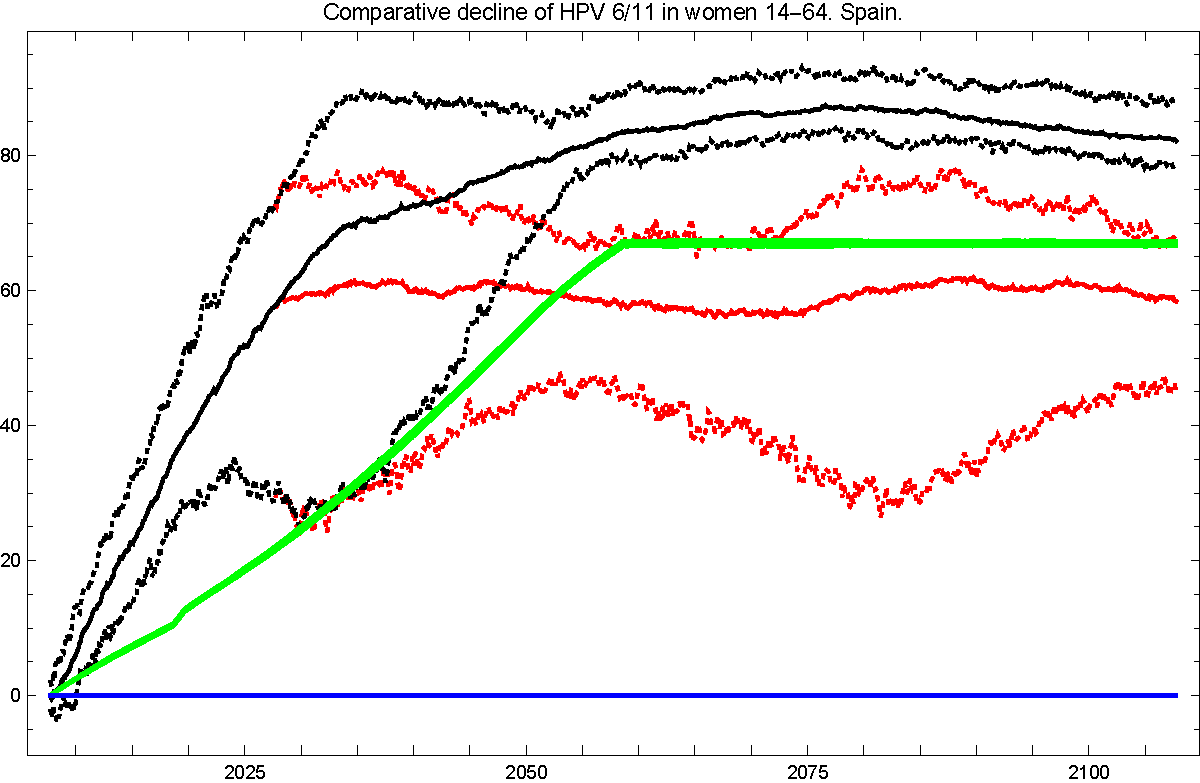
\includegraphics[width=0.5\linewidth]{IMGs/5.-Caida_brusca/Decl_muj_14_64_verr_Caida.pdf}	& 
		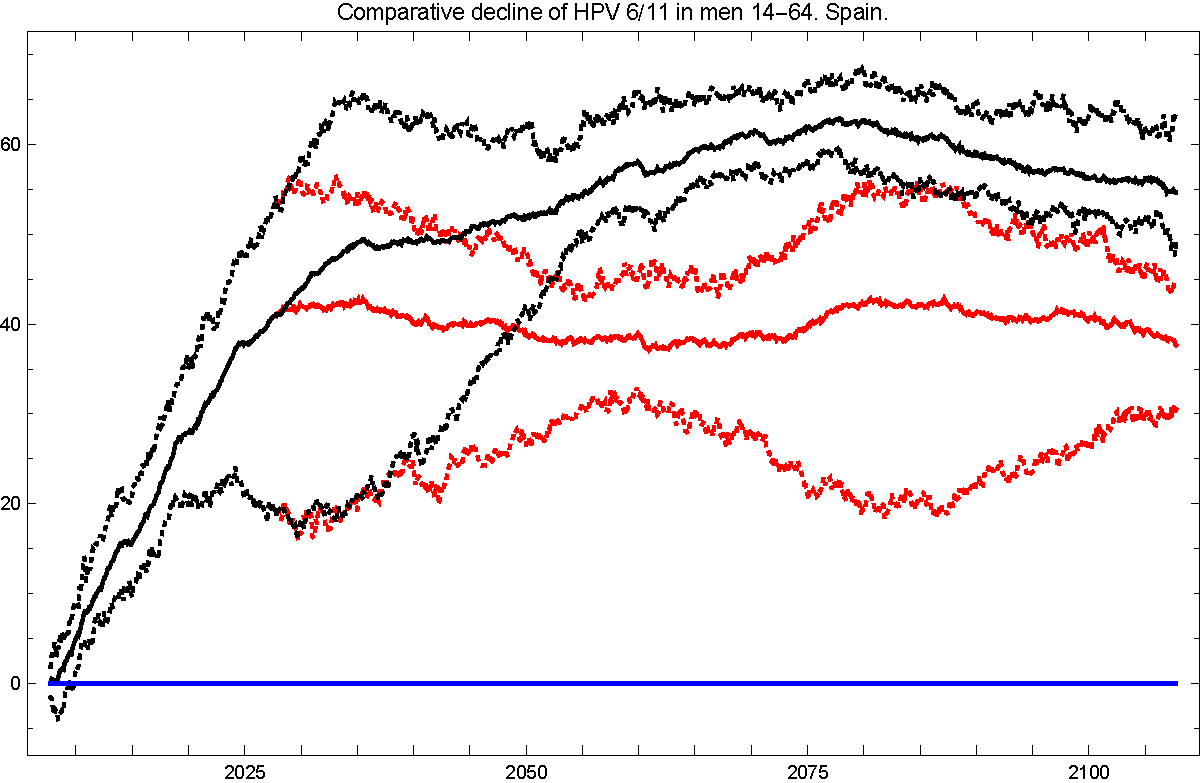
\includegraphics[width=0.5\linewidth]{IMGs/5.-Caida_brusca/Decl_hom_14_64_verr_Caida.pdf}  \\ 
		(a)	& (b) \\ 
		\multicolumn{2}{c}{ 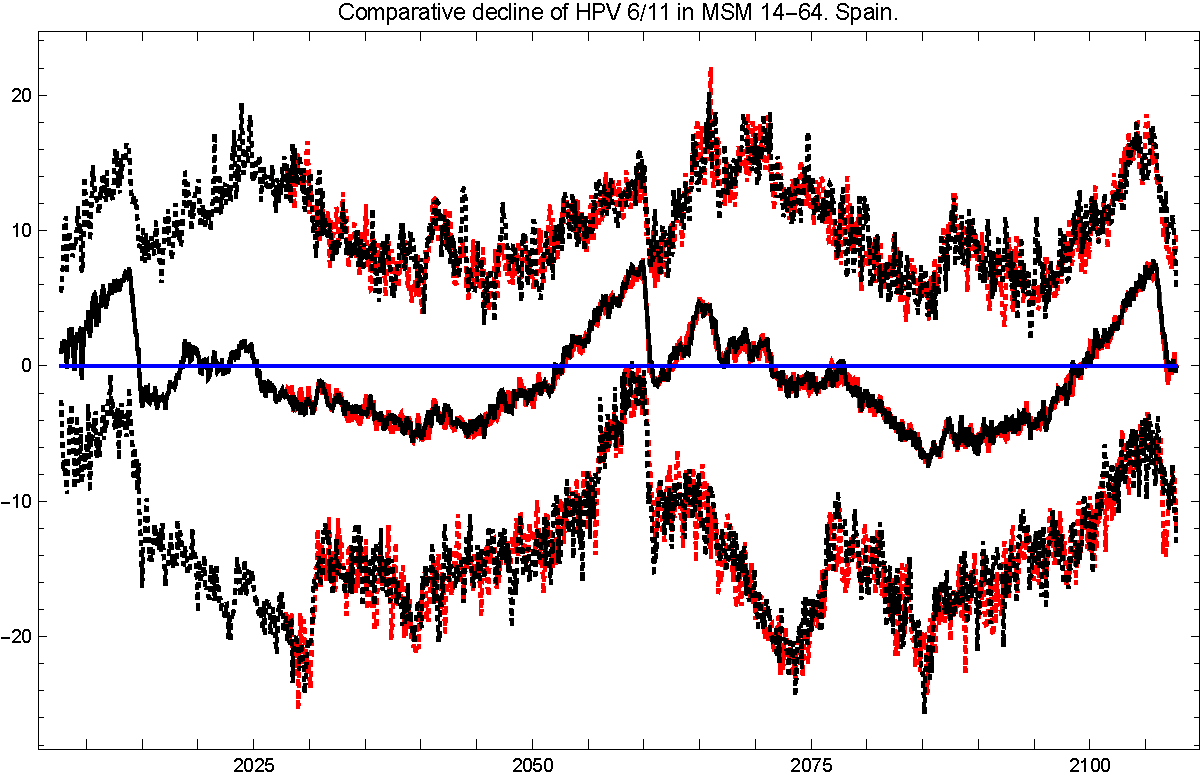
\includegraphics[width=0.5\linewidth]{IMGs/5.-Caida_brusca/Decl_MSM_14_64_verr_Caida.pdf} } \\ 
		\multicolumn{2}{c}{(c)} \\ 
	\end{tabular} 
	\caption{Comparative of the decline of HPV LR 6/11 in 14-64 years old women (a), men (b) and MSM (c) over the time, between the scenario where the effect of the vaccine is permanent (black lines, representing  the mean and the $95\%$ confidence interval) and the scenario where the effect of the vaccine disappear completely after $20$ years (red lines, representing  the mean and the $95\%$ confidence interval). As we can see, for women and men, the latter stabilizes in levels of decline about $20\%$ less, in average, than the case where the vaccine protects permanently. For MSM there are not changes between both scenarios.}
	\label{fig:dropLRESP}
\end{figure}

Now, in Figure \ref{fig:dropHRESP}, we can see an analogous comparative for the decline of HPV oncogenic HR between the mentioned scenarios: permanent protection and the drop of the protection after $20$ years. The graphs are very similar to the ones in Figure \ref{fig:dropLRESP} with the only change that the difference between the levels of decline are higher. The results for MSM are almost identical, what supports that there is not herd immunity effect on them.

\begin{figure}[!]
	\centering
	\begin{tabular}{cc}
		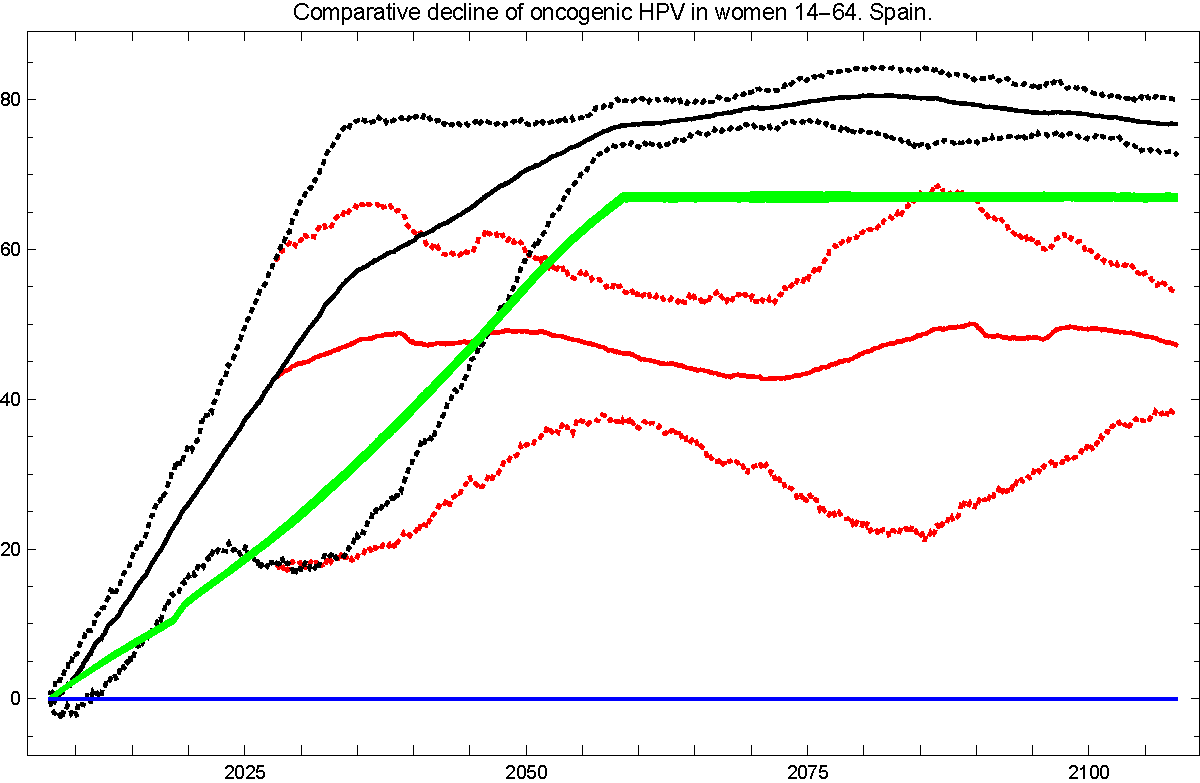
\includegraphics[width=0.5\linewidth]{IMGs/5.-Caida_brusca/Decl_muj_14_64_onco_Caida.pdf}	& 
		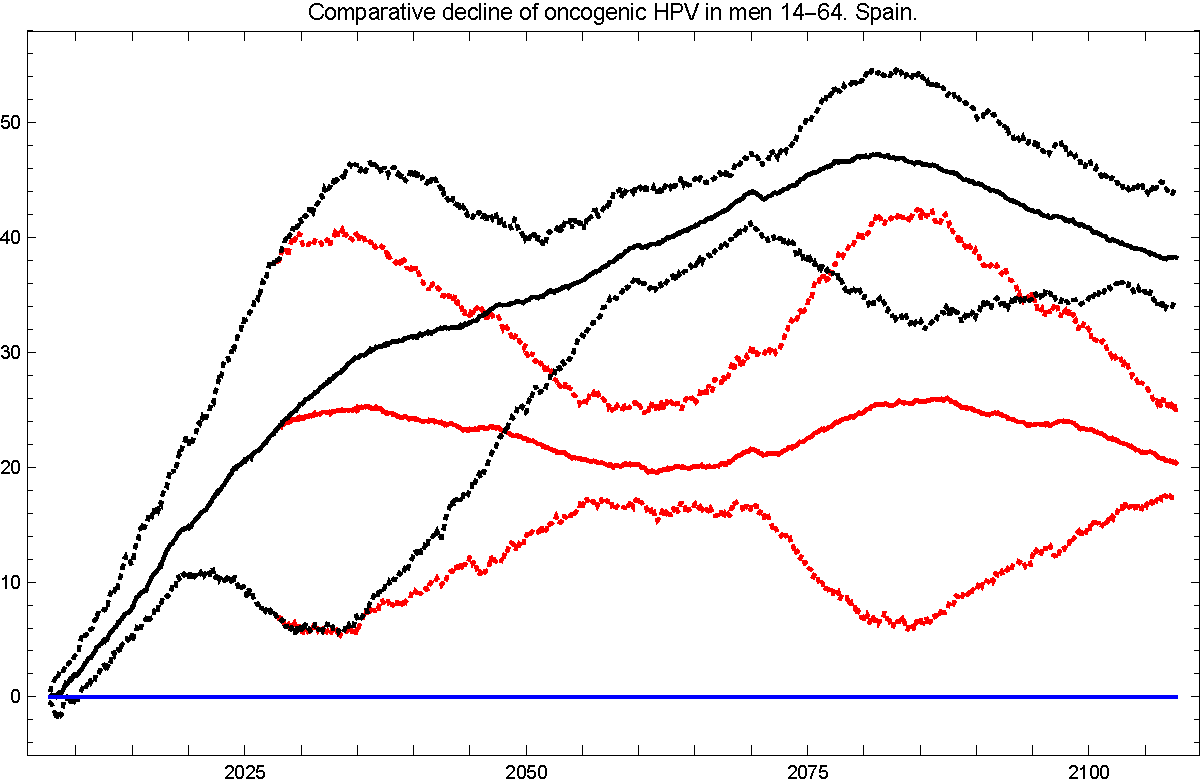
\includegraphics[width=0.5\linewidth]{IMGs/5.-Caida_brusca/Decl_hom_14_64_onco_Caida.pdf}  \\ 
		(a)	& (b) \\ 
		\multicolumn{2}{c}{ 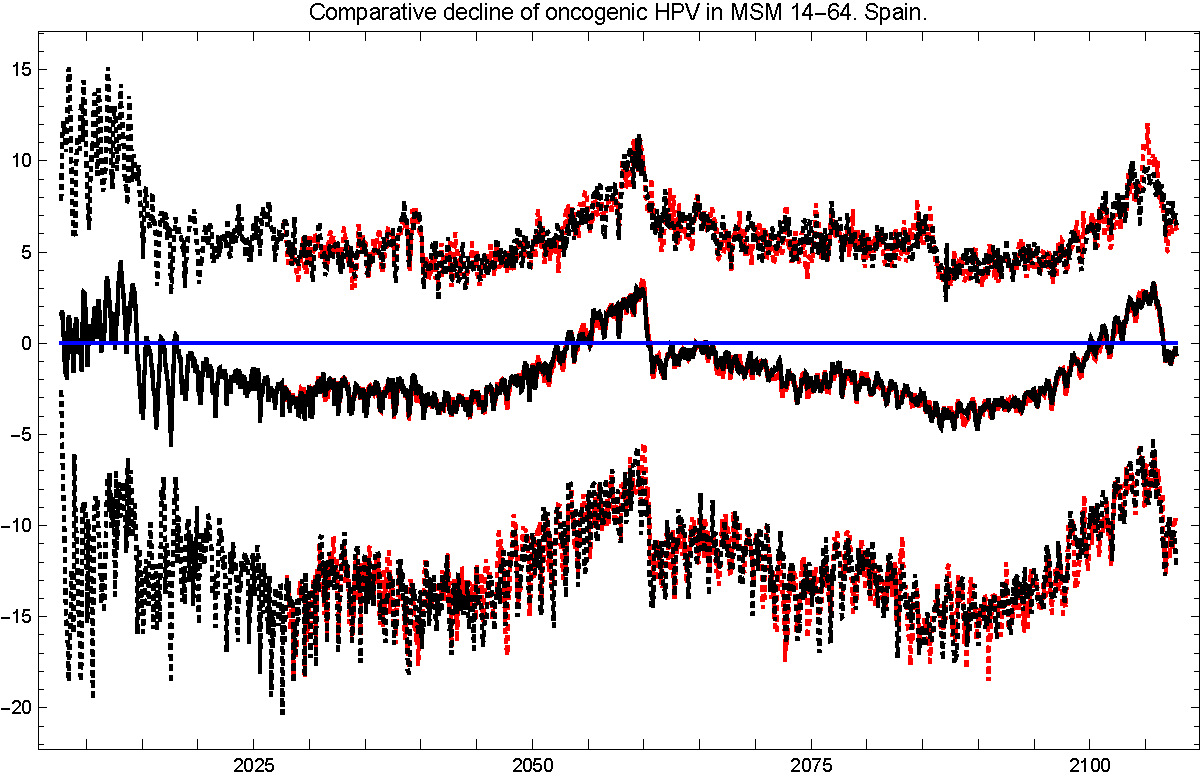
\includegraphics[width=0.5\linewidth]{IMGs/5.-Caida_brusca/Decl_MSM_14_64_onco_Caida.pdf} } \\ 
		\multicolumn{2}{c}{(c)} \\ 
	\end{tabular} 
	\caption{Comparative of the decline of  HPV oncogenic HR infections in 14-64 years old women (a), men (b) and MSM (c) over the time, between the scenario where the effect of the vaccine is permanent (black lines, representing  the mean and the $95\%$ confidence interval) and the scenario where the effect of the vaccine disappear completely after $20$ years (red lines, representing  the mean and the $95\%$ confidence interval). The graphs are very similar to the ones in Figure \ref{fig:dropLRESP} with the only change that the difference between the levels of decline are higher. For MSM there are not changes between both scenarios.}
	\label{fig:dropHRESP}
\end{figure}

Thus, we can conclude that the longer is the vaccine protection the lower will be the drop in the decline. 

\section{Simulation of the effect of the tourism on the contagion of HPV in Spain}
In $2017$, $82$ millions of tourists visited Spain \cite{INEturismo}. These visits may have influence on the spread of HPV and this is what we are going to study in the present section.

Unfortunately, there are not available data related to the number of infections due to sexual intercourses with tourists, therefore, we are going to introduce a more or less believable scenario, skewing a bit against the vaccine. This scenario will simulate, every month, that $1\%$ of Spanish individuals aged $18-29$ years old with $4$ or more LSP have sexual intercourses with infected tourists.

To do so, we need to introduce a new feature in the computational model to simulate the effect of the tourism. First, recall that, following \cite{castellsague2012prevalence}, among the infected women, $76.03\%$ of them are infected of HPV HR, $11.72\%$ are infected of HPV LR and $12.24\%$ are infected by both, HR and LR. Also, $50.35\%$ of the HPV HR are with oncogenic types, that is, HPV 16/18/31/33/45/52/58. Furthermore, $37.075\%$ of the HPV LR are with 6/11. Then, for all individuals with $4$ or more LSP aged $18-29$ ($rnd()$ denotes a computational function that generates a random number in the interval $[0,1]$.

\begin{itemize}
	\item If $rnd()<0.01$ (the individual may be infected by a tourist) and let $x=rnd()$
	\begin{itemize}
		\item If $x < 0.7603$ the node gets infected by HPV HR. Also, if $rnd() < 0.5035$ and the individual is not vaccinated, the infection is by an oncogenic HPV HR.
		\item If $0.7603 \leq x < 0.7603 + 0.1172$ the node gets infected by HPV LR. Also, if $rnd() < 0.3707$ and the individual is not vaccinated, the infection is by HPV 6/11.
		\item If $0.7603 + 0.1172 \leq x $ the node gets infected by HPV LR and by HPV LR (coinfection). Thus, if $rnd() < 0.5035$ and the individual is not vaccinated, the infection is by an oncogenic HPV HR and $rnd() < 0.3707$ the infection is also by HPV 6/11.
	\end{itemize}
\end{itemize}

Including the above features in the computational model and performing a simulation, in the Figure \ref{fig:turismo} we can see the influence of the tourism in the HPV infections.

\begin{figure}[!]
	\centering
	\begin{tabular}{cc}
		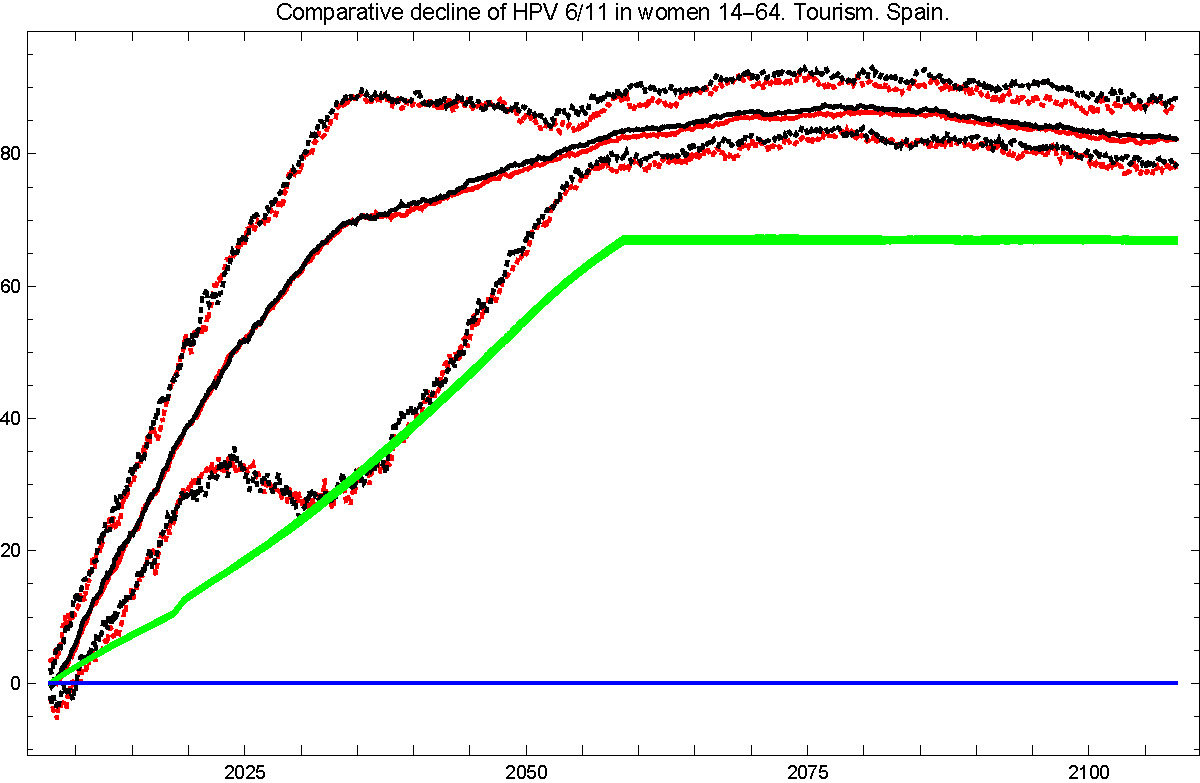
\includegraphics[width=0.5\linewidth]{IMGs/6.-Turismo/Decl_muj_14_64_verr_Turismo.pdf}	& 
		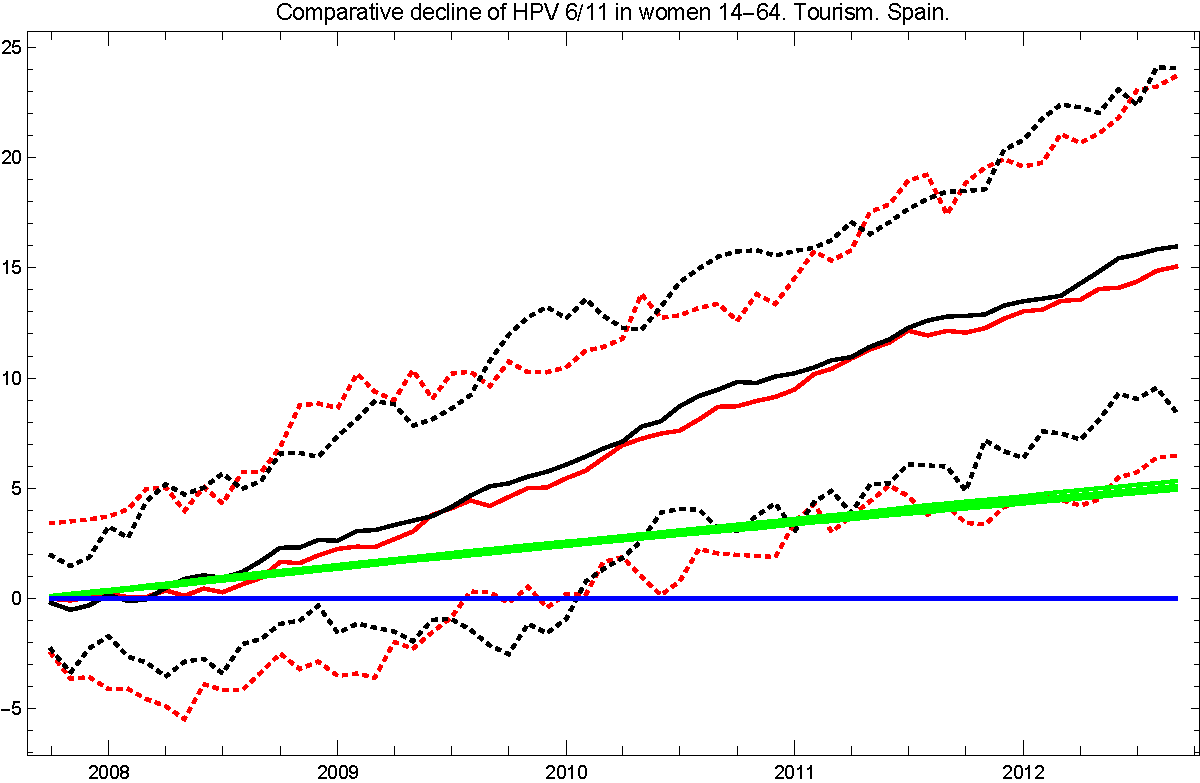
\includegraphics[width=0.5\linewidth]{IMGs/6.-Turismo/Decl_muj_14_64_verr_ZOOM_Turismo_ZOOM.pdf}  \\ 
		(a)	& (b) \\ 
		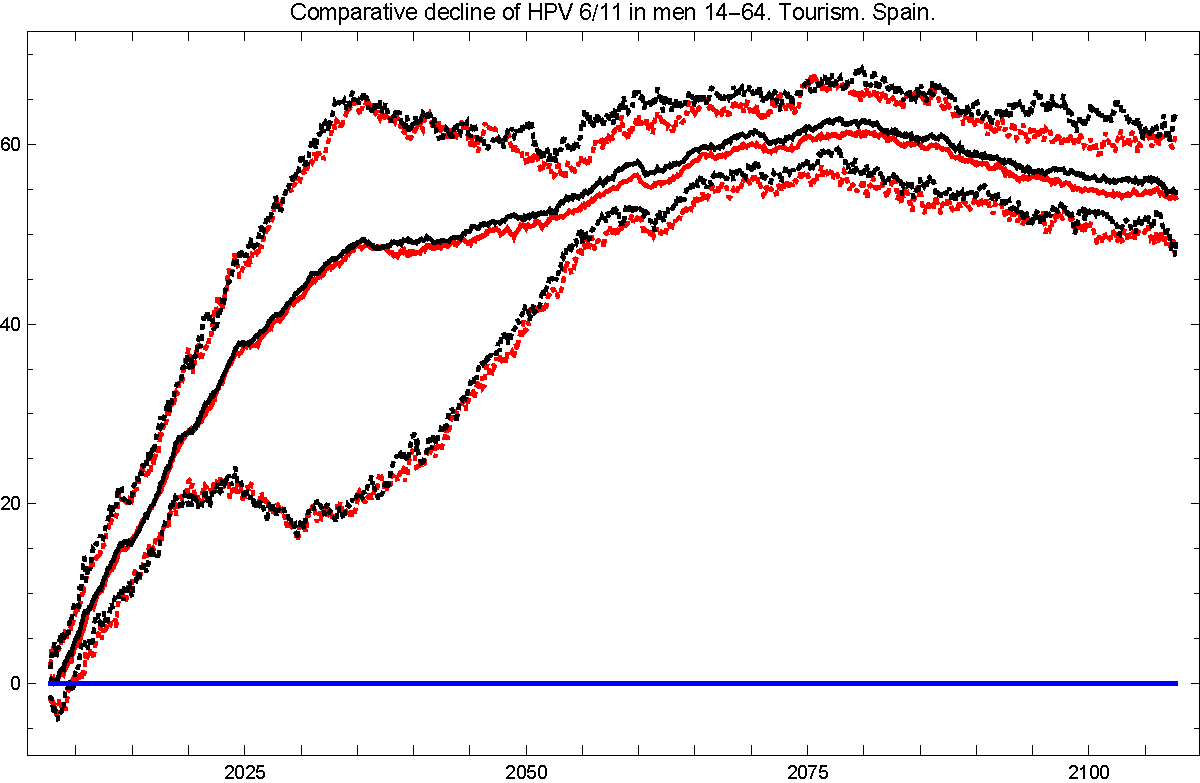
\includegraphics[width=0.5\linewidth]{IMGs/6.-Turismo//Decl_hom_14_64_verr_Turismo.pdf}	& 
		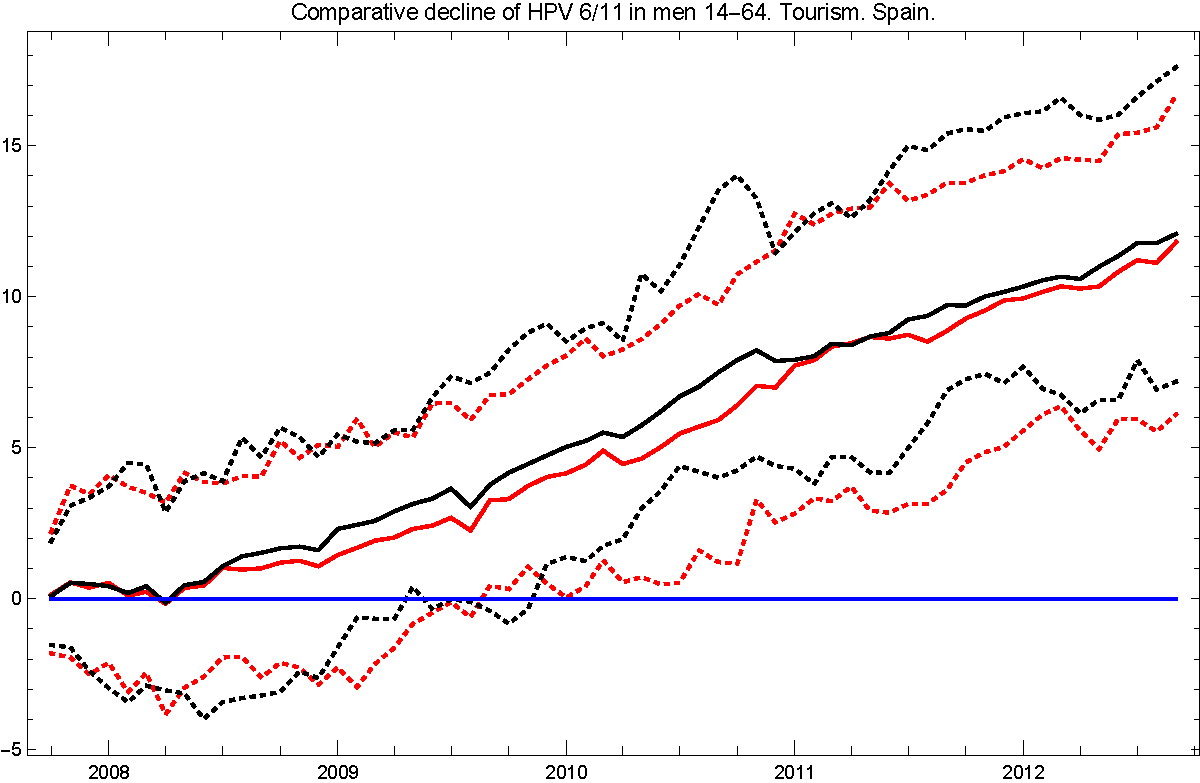
\includegraphics[width=0.5\linewidth]{IMGs/6.-Turismo/Decl_hom_14_64_verr_ZOOM_Turismo_ZOOM.pdf}  \\ 
		(c)	& (d) \\ 		
		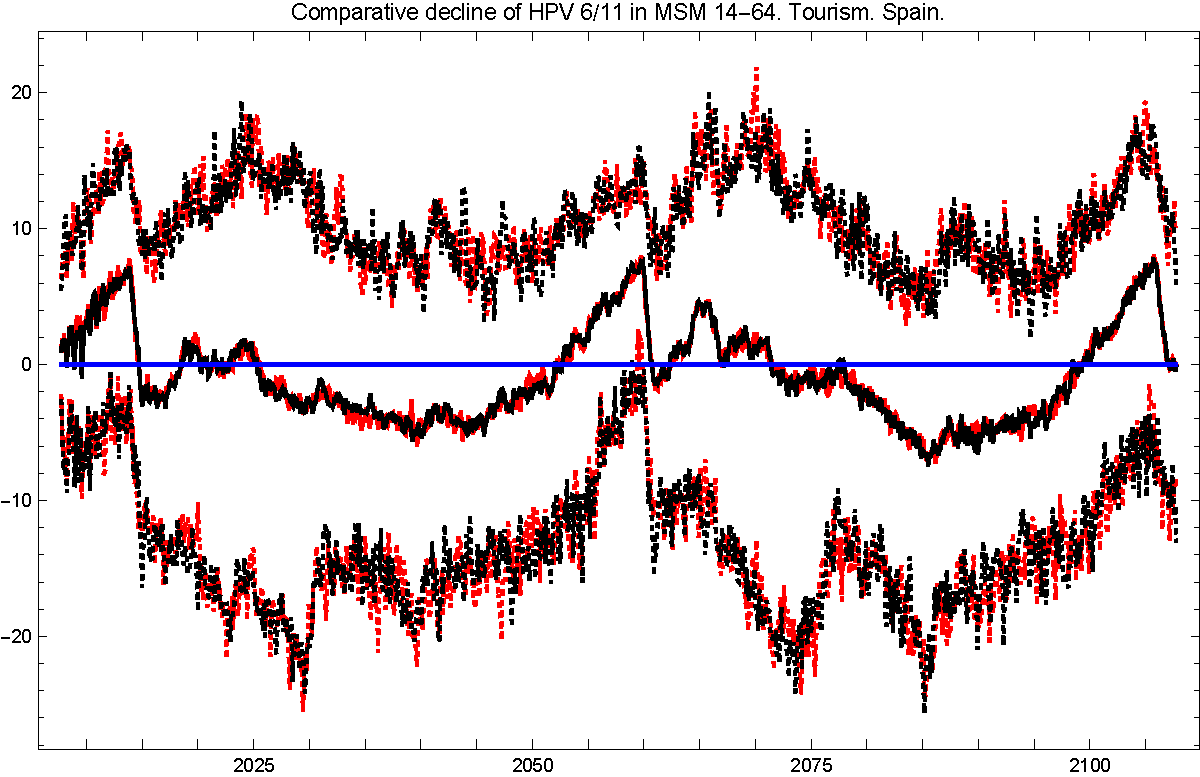
\includegraphics[width=0.5\linewidth]{IMGs/6.-Turismo/Decl_MSM_14_64_verr_Turismo.pdf}	& 
		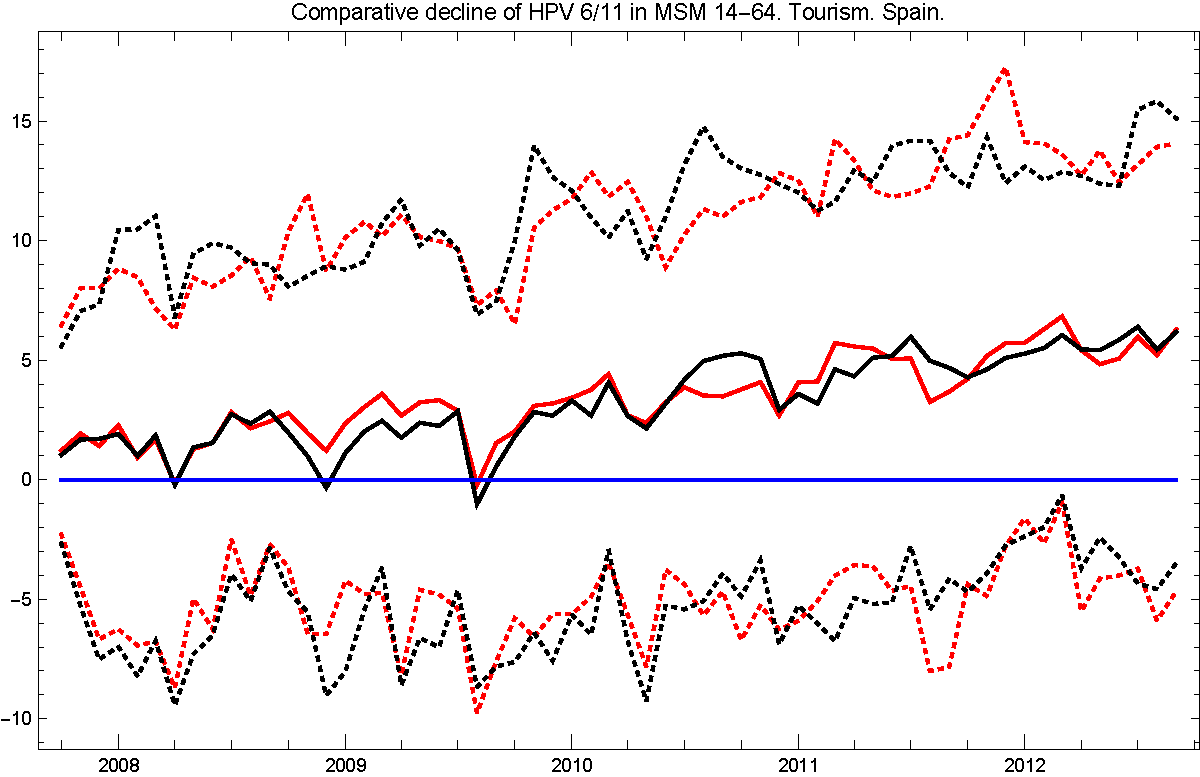
\includegraphics[width=0.5\linewidth]{IMGs/6.-Turismo/Decl_MSM_14_64_verr_ZOOM_Turismo_ZOOM.pdf}  \\ 
		(e)	& (f)
 	\end{tabular} 
	\caption{Comparative of the decline of  HPV LR 6/11 in 14-64 years old women (a), men (c) and MSM (e) over the time and a zoom of the graphs for the first five years for women (b), men (d) and MSM (f), between the non-tourism scenario (black lines, representing  the mean and the CI$95\%$) and the tourism scenario where every month $1\%$ of Spanish individuals aged $18-29$ years old with $4$ or more LSP have sexual intercourses with infected tourists (red lines, representing  the mean and the CI$95\%$). No remarkable changes appear.}
	\label{fig:turismo}
\end{figure}

Figure \ref{fig:turismo} shows that there are not remarkable differences between both scenarios including the very beginning, where there are very few girls vaccinated. Therefore, the tourism does not seem to be a factor that influences the decline the HPV 6/11. Here we do not show the same graphs for HPV oncogenic because of their similarity with the ones in Figure \ref{fig:turismo} . 
